\chapter{Patterns}
\label{sec:pats}
%%%%%%%%%%%%%%%%%%%%%%%%%%%%%%%%%%%%%%%%%%%%%%%%%%%%%%%%%
We list the individual patterns contained in CORe, together with their axioms and explanations thereof. Each axiom is listed only once (for now), i.e. some axioms pertaining to a module may be found in the axiom set listed for an earlier listed module. Schema diagrams are provided throughout, but the reader should keep in mind that while schema diagrams are very useful for understanding an ontology \cite{odp-documentation}, they are also inherently ambiguous.

\section*{Primer on Ontology Axioms}

Logical axioms are presented (mostly) in description logic notation, which can be directly translated into the Web Ontology Language OWL \cite{FOST}. We use description logic notation because it is, in the end, easier for humans to read than any of the other serializations.\footnote{Preliminary results supporting this claim can be found in \cite{ShimizuMS}.} 

Logical axioms serve many purposes in ontology modeling and engineering \cite{HitzlerK16};  in our context, the primary reason why we choose a strong axiomatization is to disambiguate the ontology.

Almost all axioms which are part of the Enslaved Ontology are of the straightforward and local types. We will now describe these types in more detail, as it will make it much easier to understand the axiomatization of the Enslaved Ontology.

\bigskip

\begin{figure}[tb]
\begin{center}
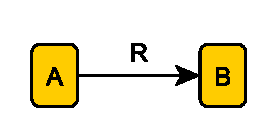
\includegraphics[width=.3\textwidth]{figures/02-ARB}
\caption{Generic node-edge-node schema diagram for explaining systematic axiomatization}\label{fig:rec-ARB}
\end{center}
\end{figure}

There is a systematic way to look at each node-edge-node triple in a schema diagram in order to decide on some of the axioms which should be added: Given a node-edge-node triple with nodes $A$ and $B$ and edge $R$ from $A$ to $B$, as depicted in Figure \ref{fig:rec-ARB}, we check all of the following axioms whether they should be included.\footnote{The OWLAx Prot\'eg\'e plug-in \cite{SarkerKH16} provides a convenient interface for adding these axioms.} We list them in natural language, see Figure \ref{fig:generic-triple-axioms-DL} for the formal versions in description logic notation, and Figure \ref{fig:generic-triple-axioms-Manchester} for the same in Manchester syntax, where we also list our names for these axioms.
\begin{compactenum}
\item $A$ is a subClass of $B$.
\item $A$ and $B$ are disjoint.
\item The domain of $R$ is $A$.
\item For every $B$ which has an inverse $R$-filler, this inverse $R$-filler is in $A$. In other words, the domain of $R$, scoped by $B$, is $A$.
\item The range of $R$ is $B$.
\item For every $A$ which has an $R$-filler, this $R$-filler is in $B$. In other words, the range of $R$, scoped by $A$, is $B$.
\item For every $A$ there has to be an $R$-filler in $B$.
\item For every $B$ there has to be an inverse $R$-filler in $A$.
\item $R$ is functional.
\item $R$ has at most one filler in $B$.
\item For every $A$ there is at most one $R$-filler.
\item For every $A$ there is at most one $R$-filler in $B$.
\item $R$ is inverse functional.
\item $R$ has at most one inverse filler in $A$.
\item For every $B$ there is at most one inverse $R$-filler.
\item For every $B$ there is at most one inverse $R$-filler in $A$.
\item An $A$ may have an $R$-filler in $B$.
\end{compactenum}

Domain and range axoims are items 2--5 in this list. Items 6 and 7 are extistential axioms. Items 8--15 are about variants of functionality and inverse functionality. All axiom types except disjointness and those utilizing inverses also apply to datatype properties.

\begin{figure}[tb]
\begin{center}
\begin{minipage}{.3\textwidth}
\begin{compactenum}
\item $A \sqsubseteq B$
\item $A\sqcap B\sqsubseteq \bot$
\item $\exists R.\top \sqsubseteq A$
\item $\exists R.B\sqsubseteq A$
\item $\top \sqsubseteq \forall R.B$ 
\item $A\sqsubseteq \forall R.B$
\end{compactenum}
\end{minipage}
\begin{minipage}{.3\textwidth}
\begin{compactenum}
\setcounter{enumi}{5}
\item $A\sqsubseteq R.B$
\item $B\sqsubseteq R^-.A$
\item $\top \sqsubseteq \mathord{\leq} 1 R.\top$ 
\item $\top \sqsubseteq \mathord{\leq} 1 R.B$
\item $A\sqsubseteq \mathord{\leq} 1 R.\top$
\item $A\sqsubseteq \mathord{\leq} 1 R.B$
\end{compactenum}
\end{minipage}
\begin{minipage}{.3\textwidth}
\begin{compactenum}
\setcounter{enumi}{10}
\item $\top \sqsubseteq \mathord{\leq} 1 R^-.\top$ 
\item $\top \sqsubseteq \mathord{\leq} 1 R^-.A$
\item $B \sqsubseteq \mathord{\leq} 1 R^-.\top$ 
\item $B \sqsubseteq \mathord{\leq} 1 R^-.A$
\item $A \sqsubseteq \mathord{\geq 0} R.B$
\end{compactenum}
\end{minipage}
\caption{Most common axioms which could be produced from a single edge $R$ between nodes $A$ and $B$ in a schema diagram: description logic notation.}\label{fig:generic-triple-axioms-DL}
\end{center}
\end{figure}

\begin{figure}[tb]
\begin{compactenum}
\item $A$ \textsf{SubClassOf} $B$ \hfill (subClass)
\item $A$ \textsf{DisjointWith} $B$ \hfill (disjointness)
\item $R$ \textsf{some} \texttt{owl:Thing} \textsf{SubClassOf} $A$ \hfill (domain)
\item $R$ \textsf{some} $B$ \textsf{SubClassOf} $A$ \hfill (scoped domain)
\item \texttt{owl:Thing} \textsf{SubClassOf} $R$ \textsf{only} $B$ \hfill (range)
\item $A$ \textsf{SubClassOf} $R$ \textsf{only} $B$ \hfill (scoped range)
\item $A$ \textsf{SubClassOf} $R$ \textsf{some} $B$ \hfill (existential)
\item $B$ \textsf{SubClassOf inverse} $R$ \textsf{some} $A$ \hfill (inverse existential)
\item \texttt{owl:Thing} \textsf{SubClassOf} $R$ \textsf{max} $1$ \texttt{owl:Thing} \hfill (functionality)
\item \texttt{owl:Thing} \textsf{SubClassOf} $R$ \textsf{max} $1$ $B$ \hfill (qualified functionality)
\item $A$ \textsf{SubClassOf} $R$ \textsf{max} $1$ \texttt{owl:Thing} \hfill (scoped functionality)
\item $A$ \textsf{SubClassOf} $R$ \textsf{max} $1$ $B$ \hfill (qualified scoped functionality)
\item \texttt{owl:Thing} \textsf{SubClassOf inverse} $R$ \textsf{max} $1$ \texttt{owl:Thing} \hfill (inverse functionality)
\item \texttt{owl:Thing} \textsf{SubClassOf inverse} $R$ \textsf{max} $1$ $A$ \hfill (inverse qualified functionality)
\item $B$ \textsf{SubClassOf inverse} $R$ \textsf{max} $1$ \texttt{owl:Thing} \hfill (inverse scoped functionality)
\item $B$ \textsf{SubClassOf inverse} $R$ \textsf{max} $1$ $A$ \hfill (inverse qualified scoped functionality)
\item $A$ \textsf{SubClassOf} $R$ \textsf{min} $0$ $B$ \hfill (structural tautology)
\end{compactenum}
\caption{Most common axioms which could be produced from a single edge $R$ between nodes $A$ and $B$ in a schema diagram: Manchester syntax.}\label{fig:generic-triple-axioms-Manchester}
\end{figure}

Structural tautologies are, indeed, tautologies, i.e., they do not carry any formal logical content. However as argued in \cite{HitzlerK16} they can help humans to understand the ontology, by indicating \emph{possible} relationships, i.e., relationships intended by the modeler which, however, cannot be cast into non-tautological axioms.

\section*{Explanations Regarding Schema Diagrams}

We utilize schema diagrams to visualize the ontology. In our experience, simple diagrams work best for this purpose. The reader needs to bear in mind, though, that these diagrams are ambiguous and incomplete visualizations of the ontology (or module), as the actual ontology (or module) is constituted by the set of axioms provided. 

We use the following visuals in our diagrams:

\begin{description}
\item[rectangular box with solid frame and orange fill:] a class
\item[rectangual box with dashed frame and blue fill:] a module, which is described in more detail elsewhere in the document
\item[rectangular box with dashed frame and purple fill:] a set of URIs constituting a controlled vocabulary
\item[oval with solid frame and yellow fill:] a data type
\item[arrow with white head and no label:] a subClass relationship
\item[arrow with solid tip and label:] a relationship (or property) other than a subClass relationship
\end{description}

%%%%%%%%%%%%%%%%%%%%%%%%%%%%%%%%%%%%%%%%%%%%%%%%%%%%%%%%
\section{Patterns Overview}
\label{ssec:pats}
%%%%%%%%%%%%%%%%%%%%%%%%%%%%
\begin{itemize}
\item Meta-patterns
\begin{itemize}
\item Explicit Typing
\item Property Reification
\item Stubs
\item Shortcuts
\end{itemize}
\item Organizing
\begin{itemize}
\item Aggregation, Bag, \& Collection
\item Sequence, List, \& Tree
\end{itemize}
\item Space, Time \& Things
\begin{itemize}
\item Spatiotemporal Extent
\item Trajectory
\item Event
\end{itemize}
\item Roles
\begin{itemize}
\item AgentRole
\item ParticipantRole
\end{itemize}
\item Descriptions \& Details
\begin{itemize}
\item Quantities and Units
\item Partonymy \& Meronymy
\item Provenance
\end{itemize}
\end{itemize}


%%%%%%%%%%%%%%%%%%%%%%%%%%%%%%%%%%%%%%%%%%%%%%%%%%%%%%%%
% patterns
\section{test}
\label{sec:test}
%%%%%%%%%%%%%%%%%%%%%%%%%%%%%%%%%%%%%%%%%%%%%%%%%%%%%%%%
\begin{figure}[h!]
\begin{center}
\includegraphics[width=.4\textwidth]{patterns/test}
\end{center}
\caption{Schema Diagram for test.
\label{fig:test}
\end{figure}
\subsection{Summary}
\label{sum:test}
%%%%%%%%%%%%%%%%%%%%%%%%%%%%
I am some summary text.

%%%%%%%%%%%%%%%%%%%%%%%%%%%%%%%%%%%%%%%%%%%%%%%%%%%%%%%%
\subsection{Axiomatization}
\label{axs:test}
%%%%%%%%%%%%%%%%%%%%%%%%%%%%
\begin{align}
\top &\sqsubseteq \forall\textsf{hasType.CVType} \\
\end{align}

%%%%%%%%%%%%%%%%%%%%%%%%%%%%%%%%%%%%%%%%%%%%%%%%%%%%%%%%
\subsection{Explanations}
\label{exp:test}
%%%%%%%%%%%%%%%%%%%%%%%%%%%%
\begin{enumerate}
\item temporary item
\end{enumerate}

%%%%%%%%%%%%%%%%%%%%%%%%%%%%%%%%%%%%%%%%%%%%%%%%%%%%%%%%
\subsection{Competency Question}
\label{cqs:test}
%%%%%%%%%%%%%%%%%%%%%%%%%%%%
\begin{enumerate}[CQ1.]
\item temporary item
\end{enumerate}

%%%%%%%%%%%%%%%%%%%%%%%%%%%%%%%%%%%%%%%%%%%%%%%%%%%%%%%%
% End Section
%%%%%%%%%%%%%%%%%%%%%%%%%%%%%%%%%%%%%%%%%%%%%%%%%%%%%%%%
%%%%%%%%%%%%%%%%%%%%%%%%%%%%%%%%%%%%%%%%%%%%%%%%%%%%%%%%